

% This document was generated by the publish-function
% from GNU Octave 4.2.1



\documentclass[10pt]{article}
\usepackage{listings}
\usepackage{mathtools}
\usepackage{amssymb}
\usepackage{graphicx}
\usepackage{hyperref}
\usepackage{xcolor}
\usepackage{titlesec}
\usepackage[utf8]{inputenc}
\usepackage[T1]{fontenc}
\usepackage{lmodern}


\lstset{
language=Octave,
numbers=none,
frame=single,
tabsize=2,
showstringspaces=false,
breaklines=true}


\titleformat*{\section}{\Huge\bfseries}
\titleformat*{\subsection}{\large\bfseries}
\renewcommand{\contentsname}{\Large\bfseries Contents}
\setlength{\parindent}{0pt}

\begin{document}

{\Huge\section*{test}}

\tableofcontents
\vspace*{4em}

\begin{lstlisting}
x = [50,100,150,200,250,300,350,400]
simulate = [0, 0, 0, 0 ,0 ,0, 0, 0]
counts = [0,0,0,0,0,0,0,0]

%%Question 1 is written in photo in the same direcotry
\end{lstlisting}
\begin{lstlisting}[language={},xleftmargin=5pt,frame=none]
x =
    50   100   150   200   250   300   350   400
simulate =
   0   0   0   0   0   0   0   0
counts =
   0   0   0   0   0   0   0   0

\end{lstlisting}


\phantomsection
\addcontentsline{toc}{section}{Test forward substitution}
\subsection*{Test forward substitution}

\begin{lstlisting}
for i = 1:8
	for j = 1:10
		test = rand(i*20);
		%while (forward(test)(3) == 0)
		%	test = rand(i*20);
		%end

		tic
		[U, flag] = forward(test);
		endtime = toc

		counts(i)= counts(i) + endtime;
	end
end
%
\end{lstlisting}
\begin{lstlisting}[language={},xleftmargin=5pt,frame=none]
flag =  1
endtime =  0.0042498
flag =  1
endtime =  0.0042329
flag =  1
endtime =  0.0043368
flag =  1
endtime =  0.0058758
flag =  1
endtime =  0.0048361
flag =  1
endtime =  0.0042009
flag =  1
endtime =  0.0041389
flag =  1
endtime =  0.0039899
flag =  1
endtime =  0.0040362
flag =  1
endtime =  0.0041132
flag =  1
endtime =  0.014833
flag =  1
endtime =  0.014871
flag =  1
endtime =  0.016727
flag =  1
endtime =  0.019560
flag =  1
endtime =  0.015555
flag =  1
endtime =  0.014888
flag =  1
endtime =  0.019803
flag =  1
endtime =  0.014593
flag =  1
endtime =  0.015477
flag =  1
endtime =  0.018319
flag =  1
endtime =  0.034587
flag =  1
endtime =  0.032622
flag =  1
endtime =  0.040407
flag =  1
endtime =  0.034827
flag =  1
endtime =  0.032379
flag =  1
endtime =  0.033831
flag =  1
endtime =  0.033748
flag =  1
endtime =  0.043568
flag =  1
endtime =  0.039036
flag =  1
endtime =  0.032889
flag =  1
endtime =  0.059444
flag =  1
endtime =  0.067199
flag =  1
endtime =  0.070407
flag =  1
endtime =  0.067760
flag =  1
endtime =  0.057627
flag =  1
endtime =  0.063768
flag =  1
endtime =  0.064667
flag =  1
endtime =  0.066244
flag =  1
endtime =  0.064352
flag =  1
endtime =  0.060937
flag =  1
endtime =  0.092533
flag =  1
endtime =  0.090458
flag =  1
endtime =  0.11238
flag =  1
endtime =  0.11149
flag =  1
endtime =  0.096846
flag =  1
endtime =  0.097383
flag =  1
endtime =  0.10189
flag =  1
endtime =  0.10571
flag =  1
endtime =  0.097954
flag =  1
endtime =  0.098705
flag =  1
endtime =  0.14948
flag =  1
endtime =  0.14766
flag =  1
endtime =  0.16020
flag =  1
endtime =  0.13466
flag =  1
endtime =  0.15080
flag =  1
endtime =  0.14715
flag =  1
endtime =  0.13720
flag =  1
endtime =  0.13601
flag =  1
endtime =  0.14087
flag =  1
endtime =  0.15029
flag =  1
endtime =  0.19438
flag =  1
endtime =  0.19140
flag =  1
endtime =  0.19618
flag =  1
endtime =  0.20625
flag =  1
endtime =  0.20566
flag =  1
endtime =  0.19215
flag =  1
endtime =  0.18397
flag =  1
endtime =  0.17988
flag =  1
endtime =  0.18091
flag =  1
endtime =  0.22108
flag =  1
endtime =  0.26778
flag =  1
endtime =  0.28603
flag =  1
endtime =  0.26009
flag =  1
endtime =  0.24413
flag =  1
endtime =  0.24940
flag =  1
endtime =  0.27213
flag =  1
endtime =  0.26749
flag =  1
endtime =  0.25152
flag =  1
endtime =  0.25011
flag =  1
endtime =  0.24553

\end{lstlisting}


\phantomsection
\addcontentsline{toc}{section}{Simulate foward decomposition the triple polynomial curve}
\subsection*{Simulate foward decomposition the triple polynomial curve}

\begin{lstlisting}
%
[p, E] = polyfit(x, counts, 2)

simulated_x = linspace(50,500)
simulate = polyval(p, simulated_x)


plot(x, counts, 'x')
hold on
plot(simulated_x, simulate)
hold off

%
\end{lstlisting}
\begin{lstlisting}[language={},xleftmargin=5pt,frame=none]
p =
   1.6449e-05  -1.5458e-04   1.2976e-02
E =
  scalar structure containing the fields:
    yf =
     Columns 1 through 6:
       0.046370   0.162010   0.359897   0.640029   1.002408   1.447034
     Columns 7 and 8:
       1.973905   2.583023
    X =
         2500       50        1
        10000      100        1
        22500      150        1
        40000      200        1
        62500      250        1
        90000      300        1
       122500      350        1
       160000      400        1
    R =
      -2.3415e+05  -6.9187e+02  -2.1781e+00
       0.0000e+00  -1.7696e+02  -1.6559e+00
       0.0000e+00   0.0000e+00   7.1677e-01
    C =
       9.5238e-10  -4.2857e-07   3.5714e-05
      -4.2857e-07   2.0238e-04  -1.8214e-02
       3.5714e-05  -1.8214e-02   1.9464e+00
    df =  5
    normr =  0.026356
simulated_x =
 Columns 1 through 8:
    50.000    54.545    59.091    63.636    68.182    72.727    77.273    81.818
 Columns 9 through 16:
    86.364    90.909    95.455   100.000   104.545   109.091   113.636   118.182
 Columns 17 through 24:
   122.727   127.273   131.818   136.364   140.909   145.455   150.000   154.545
 Columns 25 through 32:
   159.091   163.636   168.182   172.727   177.273   181.818   186.364   190.909
 Columns 33 through 40:
   195.455   200.000   204.545   209.091   213.636   218.182   222.727   227.273
 Columns 41 through 48:
   231.818   236.364   240.909   245.455   250.000   254.545   259.091   263.636
 Columns 49 through 56:
   268.182   272.727   277.273   281.818   286.364   290.909   295.455   300.000
 Columns 57 through 64:
   304.545   309.091   313.636   318.182   322.727   327.273   331.818   336.364
 Columns 65 through 72:
   340.909   345.455   350.000   354.545   359.091   363.636   368.182   372.727
 Columns 73 through 80:
   377.273   381.818   386.364   390.909   395.455   400.000   404.545   409.091
 Columns 81 through 88:
   413.636   418.182   422.727   427.273   431.818   436.364   440.909   445.455
 Columns 89 through 96:
   450.000   454.545   459.091   463.636   468.182   472.727   477.273   481.818
 Columns 97 through 100:
   486.364   490.909   495.455   500.000
simulate =
 Columns 1 through 7:
   0.046370   0.053484   0.061278   0.069752   0.078905   0.088738   0.099251
 Columns 8 through 14:
   0.110443   0.122315   0.134867   0.148099   0.162010   0.176601   0.191872
 Columns 15 through 21:
   0.207823   0.224453   0.241763   0.259752   0.278422   0.297771   0.317800
 Columns 22 through 28:
   0.338508   0.359897   0.381965   0.404712   0.428140   0.452247   0.477034
 Columns 29 through 35:
   0.502500   0.528647   0.555473   0.582979   0.611164   0.640029   0.669574
 Columns 36 through 42:
   0.699799   0.730703   0.762287   0.794551   0.827495   0.861118   0.895421
 Columns 43 through 49:
   0.930404   0.966066   1.002408   1.039430   1.077132   1.115513   1.154574
 Columns 50 through 56:
   1.194315   1.234735   1.275836   1.317615   1.360075   1.403214   1.447034
 Columns 57 through 63:
   1.491532   1.536711   1.582569   1.629107   1.676325   1.724222   1.772799
 Columns 64 through 70:
   1.822056   1.871993   1.922609   1.973905   2.025881   2.078536   2.131871
 Columns 71 through 77:
   2.185886   2.240581   2.295955   2.352009   2.408743   2.466157   2.524250
 Columns 78 through 84:
   2.583023   2.642475   2.702608   2.763420   2.824912   2.887083   2.949935
 Columns 85 through 91:
   3.013466   3.077676   3.142567   3.208137   3.274387   3.341316   3.408926
 Columns 92 through 98:
   3.477215   3.546183   3.615832   3.686160   3.757168   3.828856   3.901223
 Columns 99 and 100:
   3.974270   4.047997

\end{lstlisting}
\begin{figure}[!ht]
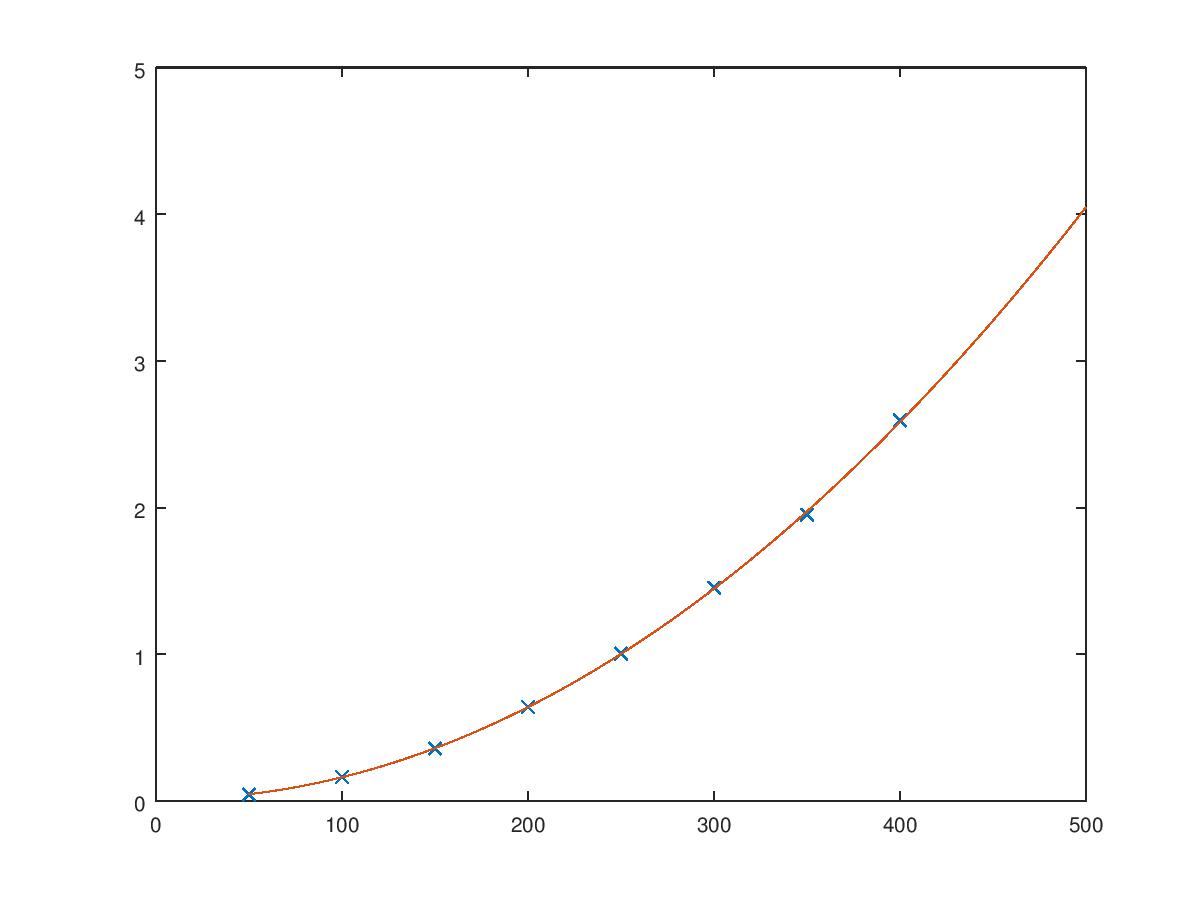
\includegraphics[width=\textwidth]{test-1.jpg}
\end{figure}


\phantomsection
\addcontentsline{toc}{section}{Test the LU decomposition}
\subsection*{Test the LU decomposition}

\begin{lstlisting}
%
for i = 1:8
	for j = 1:10
		test = rand(i*20);
		% while (LU(test)(3) == 0)
		% 	test = rand(i*20);
		%end

		tic
		[L, U, flag] = LU(test);
		endtime = toc

		counts(i)= counts(i) + endtime;
	end
end

%
\end{lstlisting}
\begin{lstlisting}[language={},xleftmargin=5pt,frame=none]
flag =  1
warning: LU: some elements in list of return values are undefined
endtime =    2.2721e-04
flag =  1
warning: LU: some elements in list of return values are undefined
endtime =    8.8930e-05
flag =  1
warning: LU: some elements in list of return values are undefined
endtime =    8.2016e-05
flag =  1
warning: LU: some elements in list of return values are undefined
endtime =    8.1062e-05
flag =  1
warning: LU: some elements in list of return values are undefined
endtime =    8.0109e-05
flag =  1
warning: LU: some elements in list of return values are undefined
endtime =    7.7963e-05
flag =  1
warning: LU: some elements in list of return values are undefined
endtime =    7.7963e-05
flag =  1
warning: LU: some elements in list of return values are undefined
endtime =    7.8917e-05
flag =  1
warning: LU: some elements in list of return values are undefined
endtime =    7.7009e-05
flag =  1
warning: LU: some elements in list of return values are undefined
endtime =    7.7009e-05
flag =  1
warning: LU: some elements in list of return values are undefined
endtime =    7.8201e-05
flag =  1
warning: LU: some elements in list of return values are undefined
endtime =    9.0122e-05
flag =  1
warning: LU: some elements in list of return values are undefined
endtime =    1.3995e-04
flag =  1
warning: LU: some elements in list of return values are undefined
endtime =    1.2112e-04
flag =  1
warning: LU: some elements in list of return values are undefined
endtime =    1.1802e-04
flag =  1
warning: LU: some elements in list of return values are undefined
endtime =    9.1076e-05
flag =  1
warning: LU: some elements in list of return values are undefined
endtime =    8.7976e-05
flag =  1
warning: LU: some elements in list of return values are undefined
endtime =    7.7009e-05
flag =  1
warning: LU: some elements in list of return values are undefined
endtime =    7.7963e-05
flag =  1
warning: LU: some elements in list of return values are undefined
endtime =    7.7009e-05
flag =  1
warning: LU: some elements in list of return values are undefined
endtime =    7.7009e-05
flag =  1
warning: LU: some elements in list of return values are undefined
endtime =    7.8201e-05
flag =  1
warning: LU: some elements in list of return values are undefined
endtime =    7.7009e-05
flag =  1
warning: LU: some elements in list of return values are undefined
endtime =    7.6056e-05
flag =  1
warning: LU: some elements in list of return values are undefined
endtime =    7.7009e-05
flag =  1
warning: LU: some elements in list of return values are undefined
endtime =    7.5817e-05
flag =  1
warning: LU: some elements in list of return values are undefined
endtime =    7.7009e-05
flag =  1
warning: LU: some elements in list of return values are undefined
endtime =    7.7009e-05
flag =  1
warning: LU: some elements in list of return values are undefined
endtime =    7.7009e-05
flag =  1
warning: LU: some elements in list of return values are undefined
endtime =    7.5817e-05
flag =  1
warning: LU: some elements in list of return values are undefined
endtime =    7.7963e-05
flag =  1
warning: LU: some elements in list of return values are undefined
endtime =    7.7009e-05
flag =  1
warning: LU: some elements in list of return values are undefined
endtime =    7.6056e-05
flag =  1
warning: LU: some elements in list of return values are undefined
endtime =    7.7009e-05
flag =  1
warning: LU: some elements in list of return values are undefined
endtime =    7.7009e-05
flag =  1
warning: LU: some elements in list of return values are undefined
endtime =    7.7009e-05
flag =  1
warning: LU: some elements in list of return values are undefined
endtime =    7.6056e-05
flag =  1
warning: LU: some elements in list of return values are undefined
endtime =    7.7009e-05
flag =  1
warning: LU: some elements in list of return values are undefined
endtime =    7.7009e-05
flag =  1
warning: LU: some elements in list of return values are undefined
endtime =    7.7009e-05
flag =  1
warning: LU: some elements in list of return values are undefined
endtime =    7.7009e-05
flag =  1
warning: LU: some elements in list of return values are undefined
endtime =    7.7963e-05
flag =  1
warning: LU: some elements in list of return values are undefined
endtime =    7.7009e-05
flag =  1
warning: LU: some elements in list of return values are undefined
endtime =    7.7963e-05
flag =  1
warning: LU: some elements in list of return values are undefined
endtime =    7.7009e-05
flag =  1
warning: LU: some elements in list of return values are undefined
endtime =    7.7963e-05
flag =  1
warning: LU: some elements in list of return values are undefined
endtime =    1.1492e-04
flag =  1
warning: LU: some elements in list of return values are undefined
endtime =    8.0109e-05
flag =  1
warning: LU: some elements in list of return values are undefined
endtime =    7.8917e-05
flag =  1
warning: LU: some elements in list of return values are undefined
endtime =    7.7963e-05
flag =  1
warning: LU: some elements in list of return values are undefined
endtime =    8.2970e-05
flag =  1
warning: LU: some elements in list of return values are undefined
endtime =    8.0824e-05
flag =  1
warning: LU: some elements in list of return values are undefined
endtime =    7.8917e-05
flag =  1
warning: LU: some elements in list of return values are undefined
endtime =    7.9155e-05
flag =  1
warning: LU: some elements in list of return values are undefined
endtime =    7.8201e-05
flag =  1
warning: LU: some elements in list of return values are undefined
endtime =    7.7963e-05
flag =  1
warning: LU: some elements in list of return values are undefined
endtime =    8.3923e-05
flag =  1
warning: LU: some elements in list of return values are undefined
endtime =    7.7963e-05
flag =  1
warning: LU: some elements in list of return values are undefined
endtime =    7.7963e-05
flag =  1
warning: LU: some elements in list of return values are undefined
endtime =    7.7009e-05
flag =  1
warning: LU: some elements in list of return values are undefined
endtime =    7.8917e-05
flag =  1
warning: LU: some elements in list of return values are undefined
endtime =    8.1062e-05
flag =  1
warning: LU: some elements in list of return values are undefined
endtime =    1.2517e-04
flag =  1
warning: LU: some elements in list of return values are undefined
endtime =    8.0109e-05
flag =  1
warning: LU: some elements in list of return values are undefined
endtime =    7.9155e-05
flag =  1
warning: LU: some elements in list of return values are undefined
endtime =    7.9155e-05
flag =  1
warning: LU: some elements in list of return values are undefined
endtime =    7.7963e-05
flag =  1
warning: LU: some elements in list of return values are undefined
endtime =    7.7963e-05
flag =  1
warning: LU: some elements in list of return values are undefined
endtime =    7.8917e-05
flag =  1
warning: LU: some elements in list of return values are undefined
endtime =    7.7963e-05
flag =  1
warning: LU: some elements in list of return values are undefined
endtime =    7.8917e-05
flag =  1
warning: LU: some elements in list of return values are undefined
endtime =    7.7963e-05
flag =  1
warning: LU: some elements in list of return values are undefined
endtime =    7.9870e-05
flag =  1
warning: LU: some elements in list of return values are undefined
endtime =    7.8917e-05
flag =  1
warning: LU: some elements in list of return values are undefined
endtime =    7.7963e-05
flag =  1
warning: LU: some elements in list of return values are undefined
endtime =    7.7963e-05
flag =  1
warning: LU: some elements in list of return values are undefined
endtime =    7.8917e-05
flag =  1
warning: LU: some elements in list of return values are undefined
endtime =    7.8917e-05
flag =  1
warning: LU: some elements in list of return values are undefined
endtime =    7.8917e-05
flag =  1
warning: LU: some elements in list of return values are undefined
endtime =    7.8917e-05

\end{lstlisting}


\phantomsection
\addcontentsline{toc}{section}{Simulate LU decomposition the triple polynomial curve}
\subsection*{Simulate LU decomposition the triple polynomial curve}

\begin{lstlisting}
%
[p, E] = polyfit(x, counts, 3)

simulated_x = linspace(50,500)
simulate = polyval(p, simulated_x)


plot(x, counts, 'x')
hold on
plot(simulated_x, simulate)

%
\end{lstlisting}
\begin{lstlisting}[language={},xleftmargin=5pt,frame=none]
p =
   3.0419e-09   1.4399e-05   2.3526e-04  -4.8064e-03
E =
  scalar structure containing the fields:
    yf =
     Columns 1 through 6:
       0.043335   0.165753   0.364729   0.642545   1.001483   1.443823
     Columns 7 and 8:
       1.971848   2.587838
    X =
         125000       2500         50          1
        1000000      10000        100          1
        3375000      22500        150          1
        8000000      40000        200          1
       15625000      62500        250          1
       27000000      90000        300          1
       42875000     122500        350          1
       64000000     160000        400          1
    R =
      -8.3569e+07  -2.3101e+05  -6.5604e+02  -1.9385e+00
       0.0000e+00  -3.8225e+04  -2.7338e+02  -1.6270e+00
       0.0000e+00   0.0000e+00  -6.9789e+01  -1.1960e+00
       0.0000e+00   0.0000e+00   0.0000e+00   4.0584e-01
    C =
       1.0774e-13  -7.2727e-11   1.3872e-08  -6.6667e-07
      -7.2727e-11   5.0043e-08  -9.7922e-06   4.8571e-04
       1.3872e-08  -9.7922e-06   1.9884e-03  -1.0405e-01
      -6.6667e-07   4.8571e-04  -1.0405e-01   6.0714e+00
    df =  4
    normr =  0.024638
simulated_x =
 Columns 1 through 8:
    50.000    54.545    59.091    63.636    68.182    72.727    77.273    81.818
 Columns 9 through 16:
    86.364    90.909    95.455   100.000   104.545   109.091   113.636   118.182
 Columns 17 through 24:
   122.727   127.273   131.818   136.364   140.909   145.455   150.000   154.545
 Columns 25 through 32:
   159.091   163.636   168.182   172.727   177.273   181.818   186.364   190.909
 Columns 33 through 40:
   195.455   200.000   204.545   209.091   213.636   218.182   222.727   227.273
 Columns 41 through 48:
   231.818   236.364   240.909   245.455   250.000   254.545   259.091   263.636
 Columns 49 through 56:
   268.182   272.727   277.273   281.818   286.364   290.909   295.455   300.000
 Columns 57 through 64:
   304.545   309.091   313.636   318.182   322.727   327.273   331.818   336.364
 Columns 65 through 72:
   340.909   345.455   350.000   354.545   359.091   363.636   368.182   372.727
 Columns 73 through 80:
   377.273   381.818   386.364   390.909   395.455   400.000   404.545   409.091
 Columns 81 through 88:
   413.636   418.182   422.727   427.273   431.818   436.364   440.909   445.455
 Columns 89 through 96:
   450.000   454.545   459.091   463.636   468.182   472.727   477.273   481.818
 Columns 97 through 100:
   486.364   490.909   495.455   500.000
simulate =
 Columns 1 through 7:
   0.043335   0.051360   0.060001   0.069259   0.079136   0.089634   0.100755
 Columns 8 through 14:
   0.112499   0.124869   0.137867   0.151494   0.165753   0.180644   0.196169
 Columns 15 through 21:
   0.212330   0.229130   0.246569   0.264649   0.283372   0.302740   0.322754
 Columns 22 through 28:
   0.343417   0.364729   0.386693   0.409310   0.432582   0.456511   0.481099
 Columns 29 through 35:
   0.506346   0.532255   0.558828   0.586066   0.613972   0.642545   0.671790
 Columns 36 through 42:
   0.701706   0.732296   0.763562   0.795505   0.828128   0.861430   0.895416
 Columns 43 through 49:
   0.930085   0.965440   1.001483   1.038215   1.075638   1.113754   1.152564
 Columns 50 through 56:
   1.192071   1.232275   1.273179   1.314784   1.357092   1.400104   1.443823
 Columns 57 through 63:
   1.488251   1.533388   1.579237   1.625799   1.673076   1.721069   1.769781
 Columns 64 through 70:
   1.819214   1.869368   1.920245   1.971848   2.024178   2.077237   2.131026
 Columns 71 through 77:
   2.185547   2.240802   2.296792   2.353520   2.410987   2.469194   2.528144
 Columns 78 through 84:
   2.587838   2.648278   2.709466   2.771402   2.834090   2.897530   2.961725
 Columns 85 through 91:
   3.026676   3.092385   3.158853   3.226083   3.294076   3.362833   3.432357
 Columns 92 through 98:
   3.502648   3.573710   3.645543   3.718150   3.791531   3.865690   3.940626
 Columns 99 and 100:
   4.016343   4.092841

\end{lstlisting}
\begin{figure}[!ht]
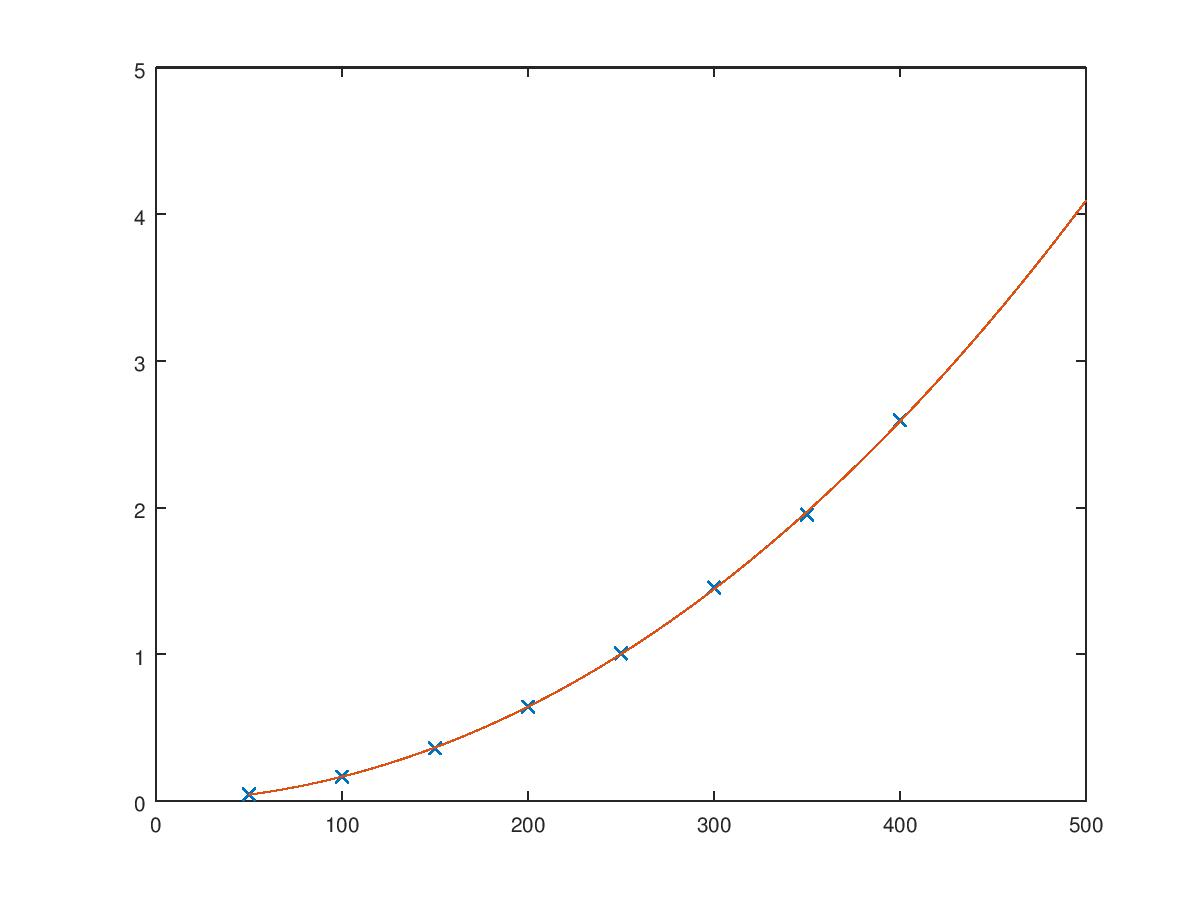
\includegraphics[width=\textwidth]{test-2.jpg}
\end{figure}


\end{document}
